\documentclass[12pt]{article}
\usepackage[margin=3cm]{geometry}
\usepackage{graphicx}
\usepackage{pgfplots}
\pgfplotsset{width=10cm,compat=1.9}

\begin{document}

\title{Relatório 2º Projeto ASA 2023/2024}
\author{Grupo: TP048 \\ Aluno: Gabriel Silva (102637)}
\date{}
\maketitle

\section{Descrição do Problema e da Solução}

\textbf{Descrição do problema:}  Dado um conjunto de pessoas e um conjunto de relações dessas pessoas, queremos estudar o pior caso de propagação de uma dada infecção em Portugal, isto é, qual o maior número de saltos que uma dada doença pode fazer. Considerou-se um pressuposto simplificador: indivíduos que se conhecem mutuamente de forma direta ou indireta, ficam infectados instantaneamente.

\textbf{Descrição da solução:} Pedir o maior número de saltos que uma dada doença pode fazer é equivalente a calcular o caminho mais longo que se pode fazer no grafo, que representa o conjunto de pessoas e relações. A lógica geral da solução é primeiro encontrar os componentes fortemente conectados no grafo usando o algoritmo de Kosaraju. Em seguida, transformar o grafo em um novo grafo onde cada SCC se torna um único nó. Fazemos isso devido à suposição simplificadora: indivíduos que se conhecem direta ou indiretamente (ciclos) são infectados instantaneamente. Por fim, calcular o caminho mais longo no novo grafo, que corresponde ao caminho mais longo no grafo original, considerando a tal suposição simplificadora.

\section{Análise Teórica}

\begin{itemize}
    \item Leitura dos dados de entrada (depende do número de relações, \(m\)): \(O(m)\)
    \item Construção do grafo (depende do número de relações, \(m\)): \(O(m)\)
    \item Aplicação do algoritmo de Kosaraju, que encontra os componentes fortemente ligados (SCCs) no grafo, e devolve um grafo de componentes: \(O(n + m)\)
        \begin{itemize}
            \item Duas procuras de profundidade que, no pior caso, visitam todos os vértices (pessoas, \(n\)) e arestas (relações, \(m\)): \(O(n + m)\)
            \item Construção do grafo de componentes: \(O(m)\)
        \end{itemize}
    \item Aplicação do algoritmo para computar o caminho mais longo: \(O(n + m)\)
        \begin{itemize}
            \item Ordenação topológica: \(O(n + m)\)
            \item Programação dinâmica: \(O(n + m)\)
        \end{itemize}
    \item Apresentação do resultado: \(O(1)\)
\end{itemize}

Complexidade global da solução: \(O(n + m)\)

\section{Avaliação Experimental dos Resultados}

\begin{table}[h]
    \centering
    \begin{tabular}{|c|c|}
        \hline
        \textbf{Complexidade} & \textbf{Tempo} \\
        \hline
        100,000 & 0.101 \\
        150,000 & 0.172 \\
        200,000 & 0.241 \\
        300,000 & 0.386 \\
        400,000 & 0.478 \\
        500,000 & 0.615 \\
        600,000 & 0.749 \\
        700,000 & 0.893 \\
        800,000 & 1.074 \\
        900,000 & 1.273 \\
        1,000,000 & 1.332 \\
        1,100,000 & 1.523 \\
        1,200,000 & 1.740 \\
        1,300,000 & 1.826 \\
        1,400,000 & 2.042 \\
        \hline
    \end{tabular}
    \caption{Complexidade f(n + m) e o Tempo (segundos)}
\end{table}

\begin{figure}[h]
    \centering
    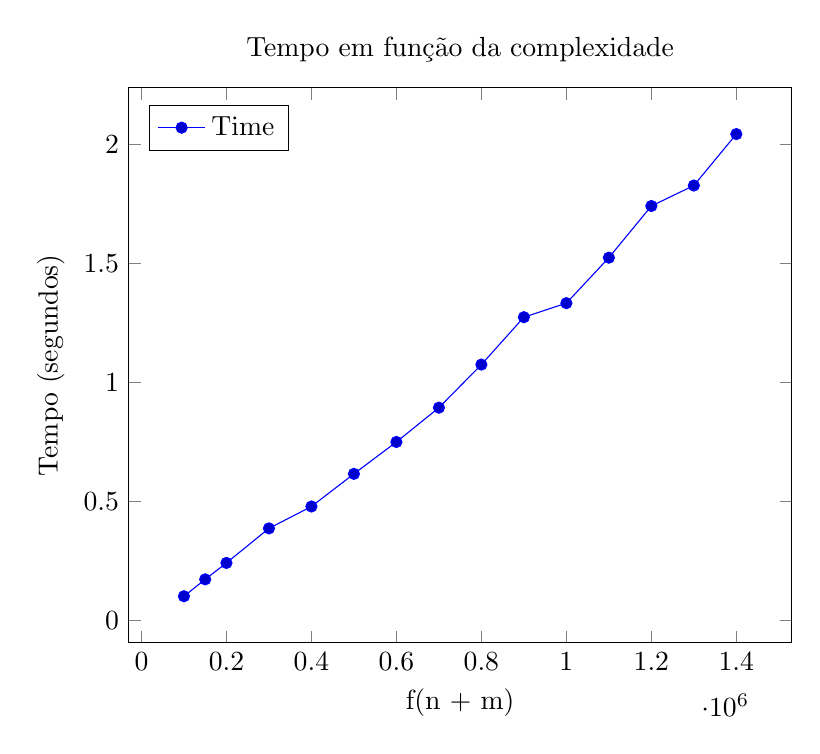
\begin{tikzpicture}
        \begin{axis}[
            xlabel={f(n + m)},
            ylabel={Tempo (segundos)},
            title={Tempo em função da complexidade},
            legend pos=north west,
        ]
            \addplot table[x=Size, y=Time, col sep=semicolon] {
                Size;Time
                100000;0.101
                150000;0.172
                200000;0.241
                300000;0.386
                400000;0.478
                500000;0.615
                600000;0.749
                700000;0.893
                800000;1.074
                900000;1.273
                1000000;1.332
                1100000;1.523
                1200000;1.740
                1300000;1.826
                1400000;2.042
            };
            \legend{Time}
        \end{axis}
    \end{tikzpicture}
\end{figure}

\end{document}
